\chapter{System Architecture}
\label{sec:system_architecture}

% ---------------------------------------------------------------
\section{Hardware Setup}
\label{sec:hardware_setup}
% ---------------------------------------------------------------

This section describes the physical components used in the experimental setup
for hand-eye calibration. The system consists of an industrial robotic
manipulator, an industrial vision sensor mounted on the robot end-effector, a
fixed-focal-length lens, and a rigid planar calibration target. The configuration
follows an \textit{eye-in-hand} setup (Section~\ref{subsec:eye_in_hand}), where
the camera is rigidly attached to the robot tool, enabling image acquisition from
multiple viewpoints through robot motion.

A summary of the main hardware components and their key parameters is provided
in Table~\ref{tab:hardware_summary}.

\begin{table}[h]
    \centering
    \caption{Summary of the experimental hardware setup.}
    \label{tab:hardware_summary}
    \begin{tabular}{lll}
        \toprule
        \textbf{Component} & \textbf{Model} & \textbf{Key parameters} \\
        \midrule
        Robot          & FANUC LR Mate 200iD
                       & 6 axes, reach 717\,mm, rep.\ $\pm$0.02\,mm \\
        Camera         & Cognex CAM-CIC-12-9C-IP67
                       & 12\,MP, 4096$\times$3000\,px, global shutter \\
        Sensor         & Sony IMX304 CMOS
                       & 1.1\,in, pixel 3.45\,$\mu$m, 12\,bit \\
        Interface      & GigE Vision (M12, PoE)
                       & up to 9\,fps at full resolution \\
        Calibration target & ChArUco board (metallic)
                       & $262 \times 402.5$\,mm,
                         sq.\ 17.5\,mm, marker 12\,mm \\  % TODO: verify exact sizes
        \bottomrule
    \end{tabular}
\end{table}

% ---------------------------------------------------------------
\subsection{Robot System}
\label{subsec:robot_system}
% ---------------------------------------------------------------

The experiments were conducted using a \textbf{FANUC LR Mate 200iD}
(Figure~\ref{fig:fanucLRMate_robot}), a compact six-axis industrial robotic manipulator
widely used in automation, assembly, and machine tending applications
\cite{siciliano2009robotics}. Its main technical specifications are:

\begin{itemize}
    \item \textbf{Degrees of freedom:} 6 rotational axes (J1--J6)
    \item \textbf{Maximum payload:} 7\,kg
    \item \textbf{Maximum reach:} 717\,mm
    \item \textbf{Pose repeatability:} $\pm$0.02\,mm (ISO~9283)
    \item \textbf{Mechanical weight:} 25\,kg
    \item \textbf{Mounting options:} floor, ceiling, wall, or angled
\end{itemize}

\begin{figure}[htbp]
	\centering
	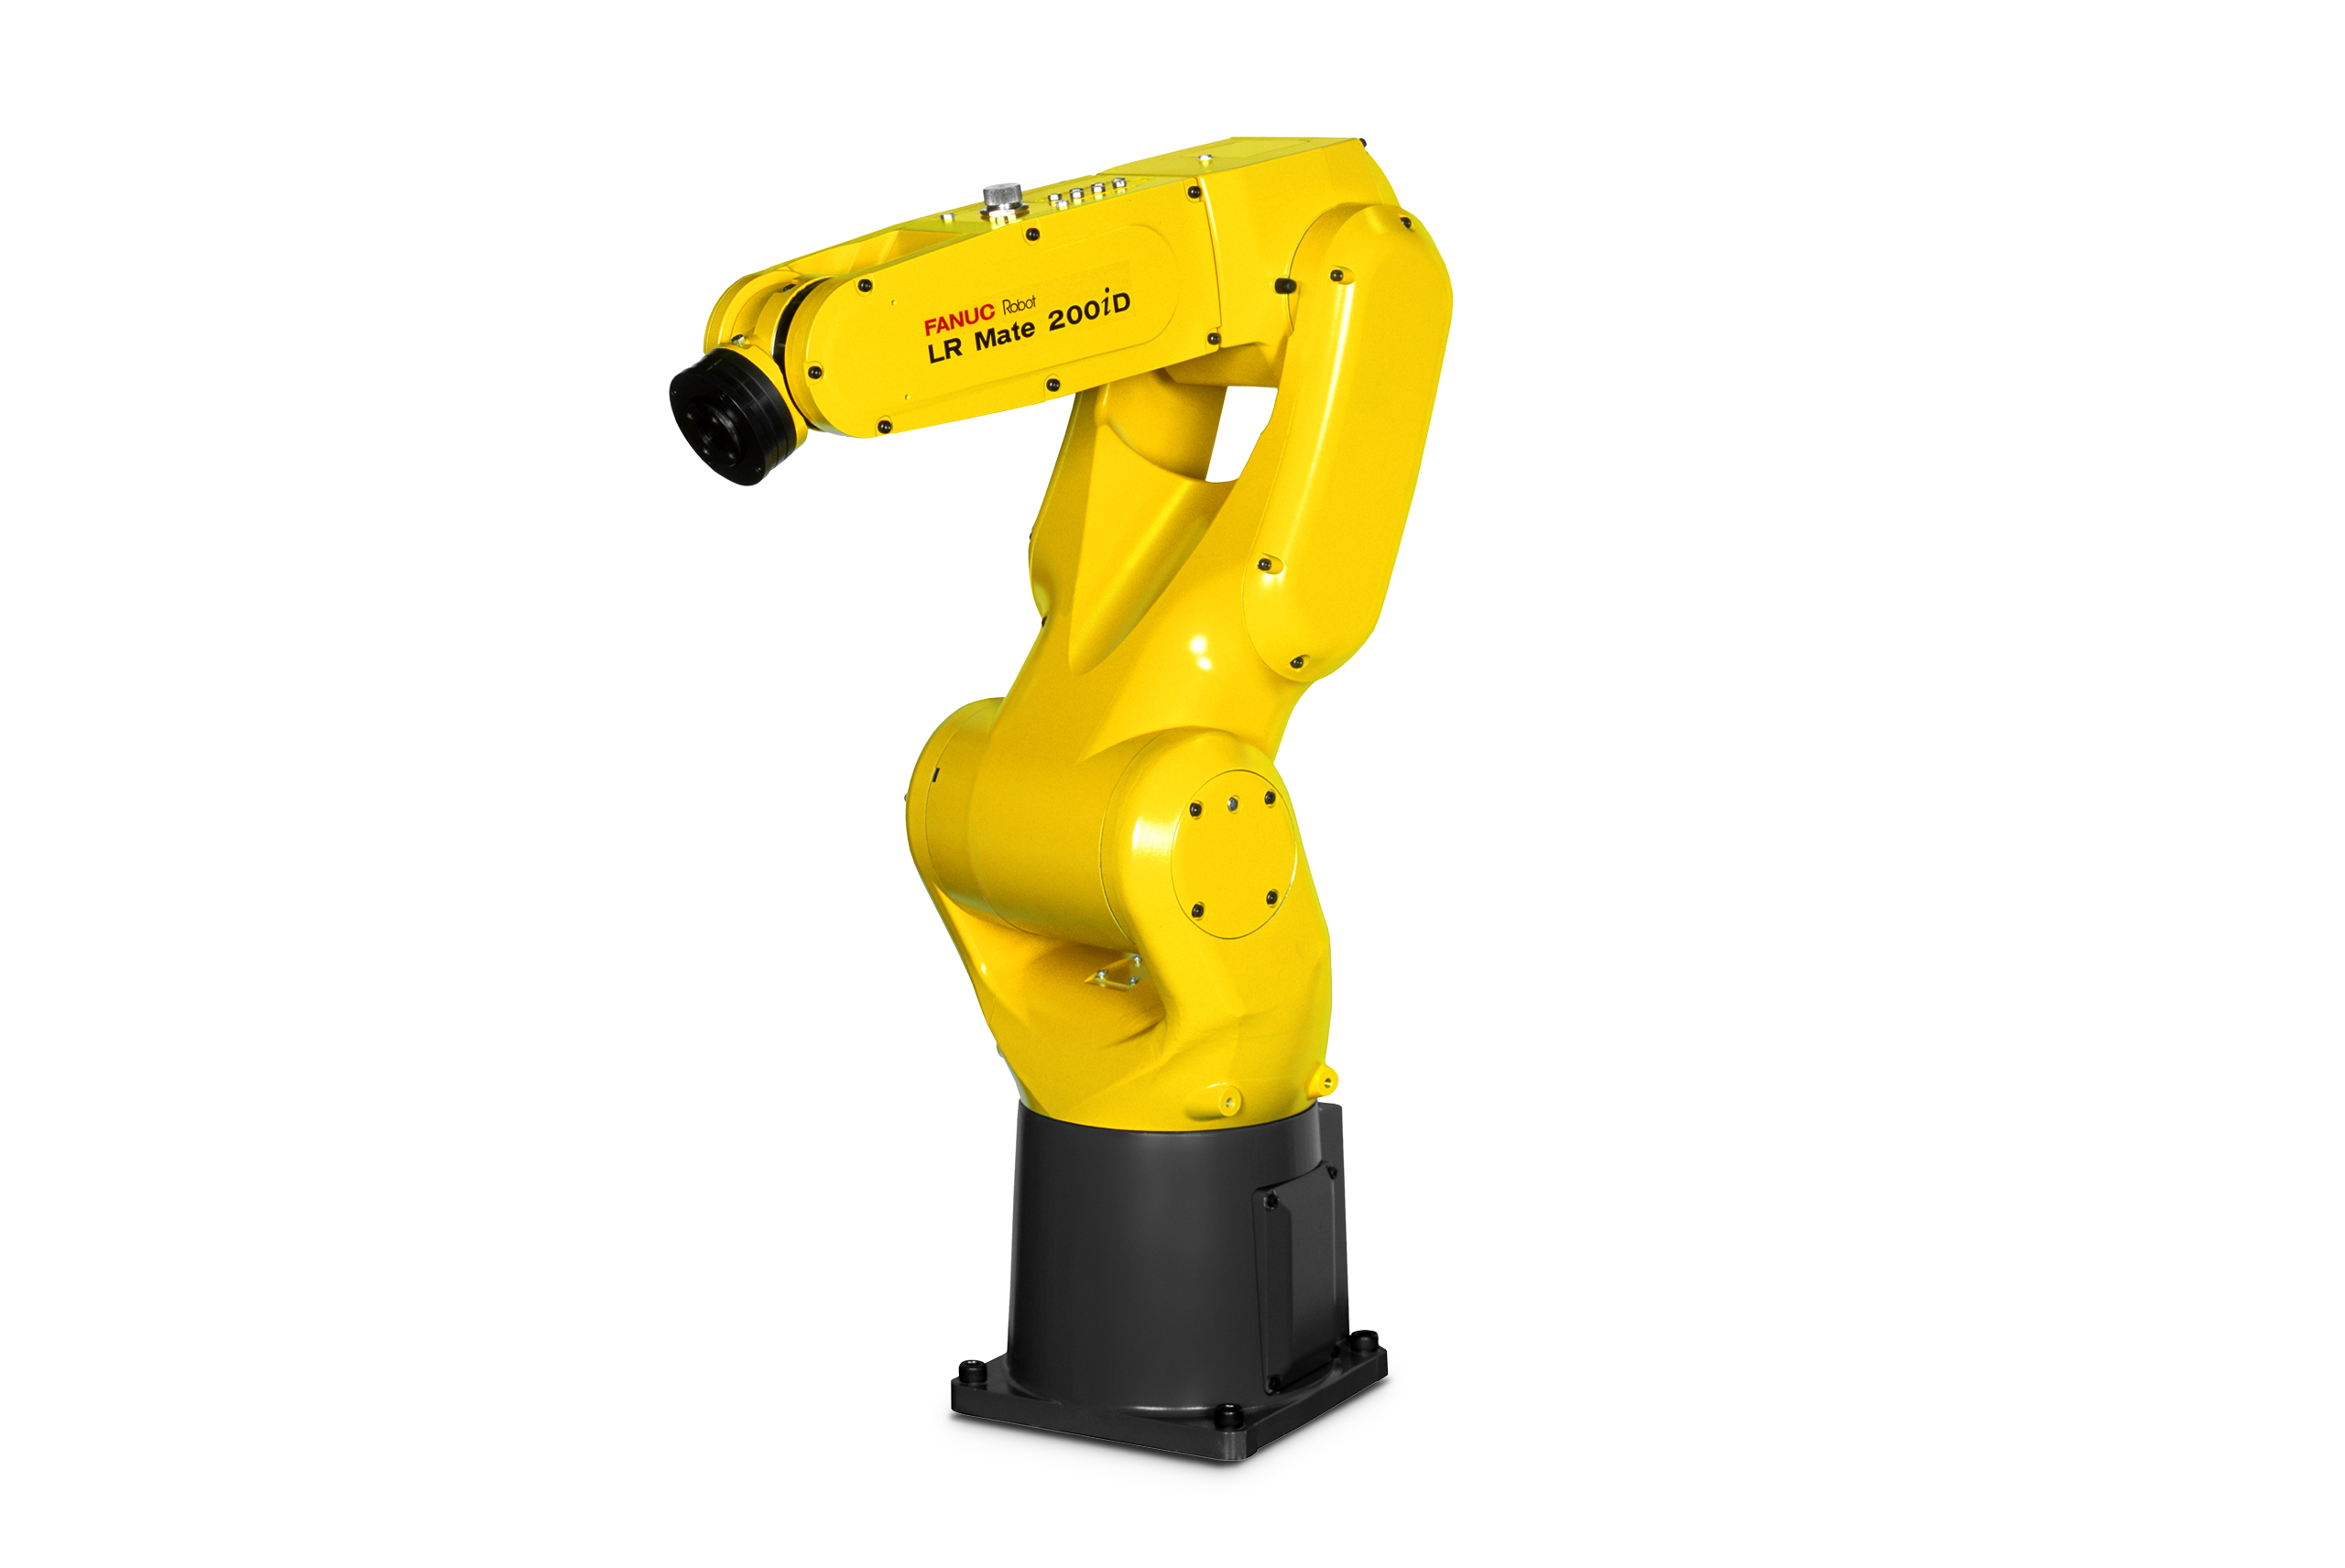
\includegraphics[width=0.55\textwidth]{images/chapter4Images/FanucLRMate200id.png}
	\caption{FANUC LR Mate 200iD robotic manipulator used in the experimental setup.}
	\label{fig:fanucLRMate_robot}
\end{figure}

\begin{figure}[htbp]
	\centering
	
	% ---------------- (a) ----------------
	\begin{subfigure}[t]{0.32\textwidth}
		\centering
		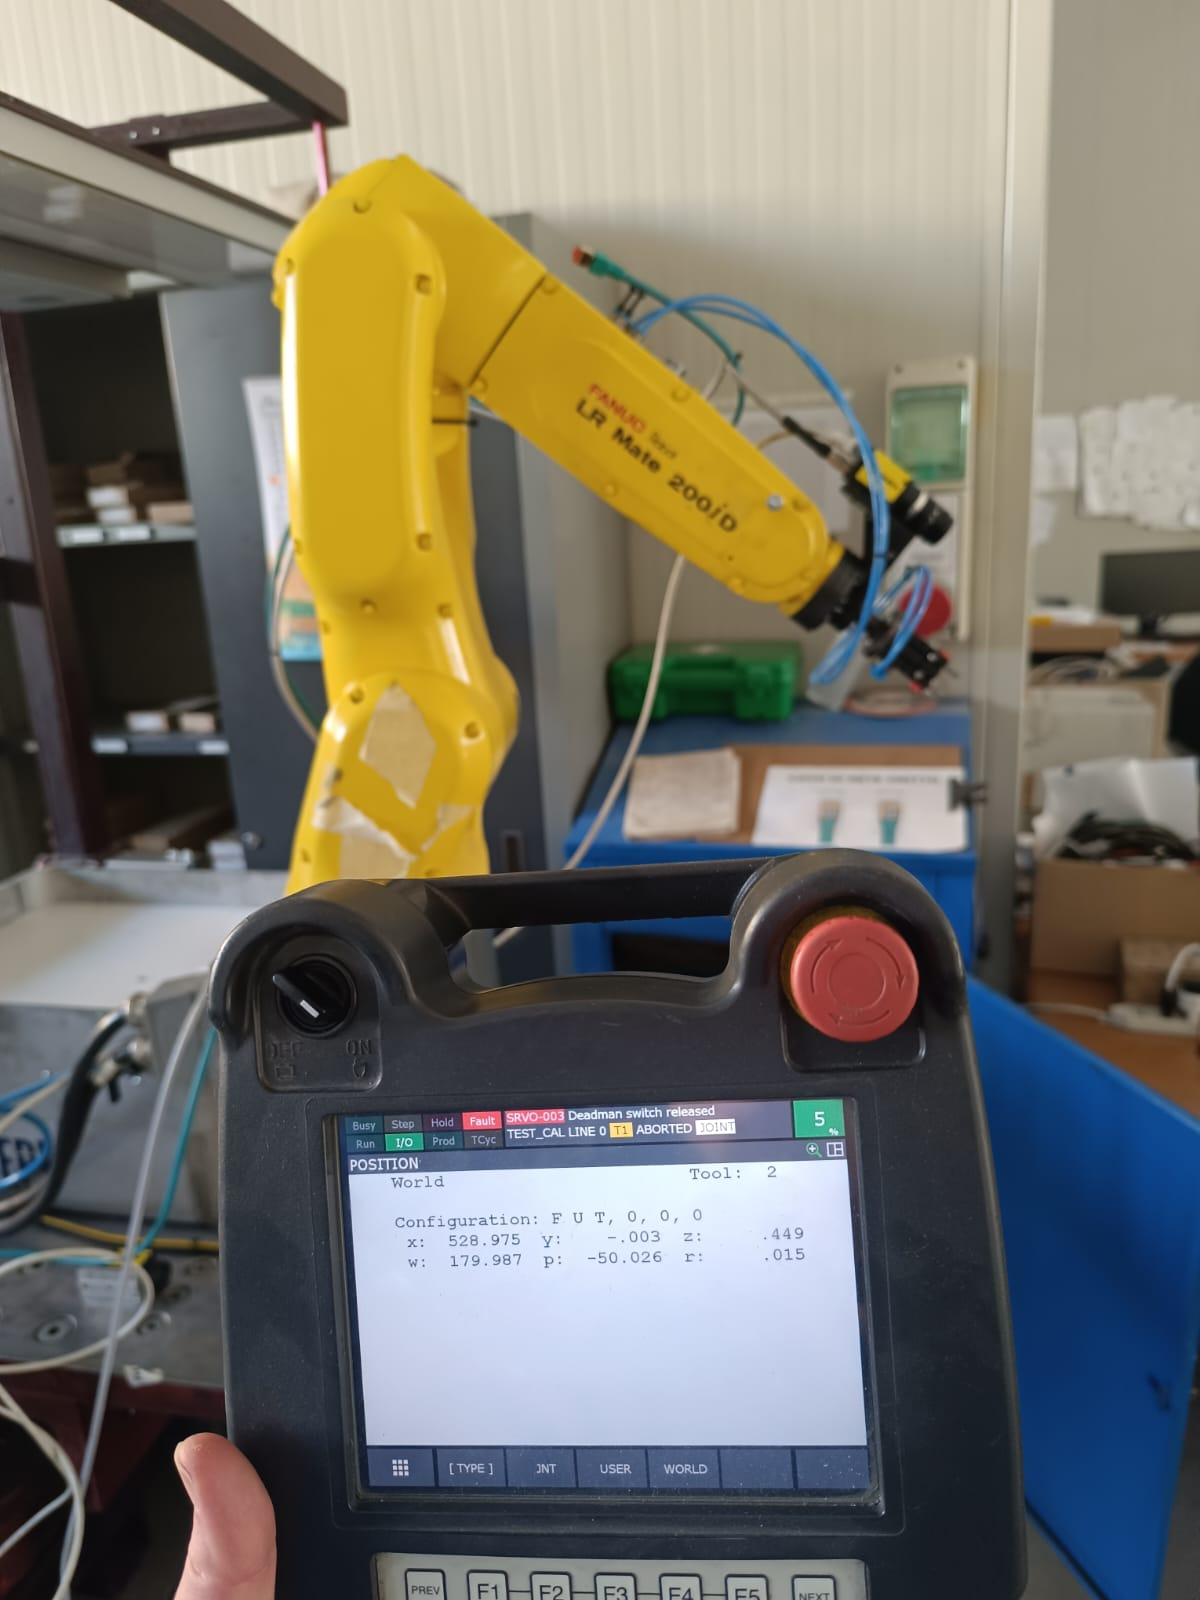
\includegraphics[width=\textwidth]{images/chapter4Images/fanuc_and_pendant.png}
		\caption{Robot with eye-in-hand camera setup.}
		\label{fig:setup_robot_close}
	\end{subfigure}
	\hfill
	
	% ---------------- (b) ----------------
	\begin{subfigure}[t]{0.32\textwidth}
		\centering
		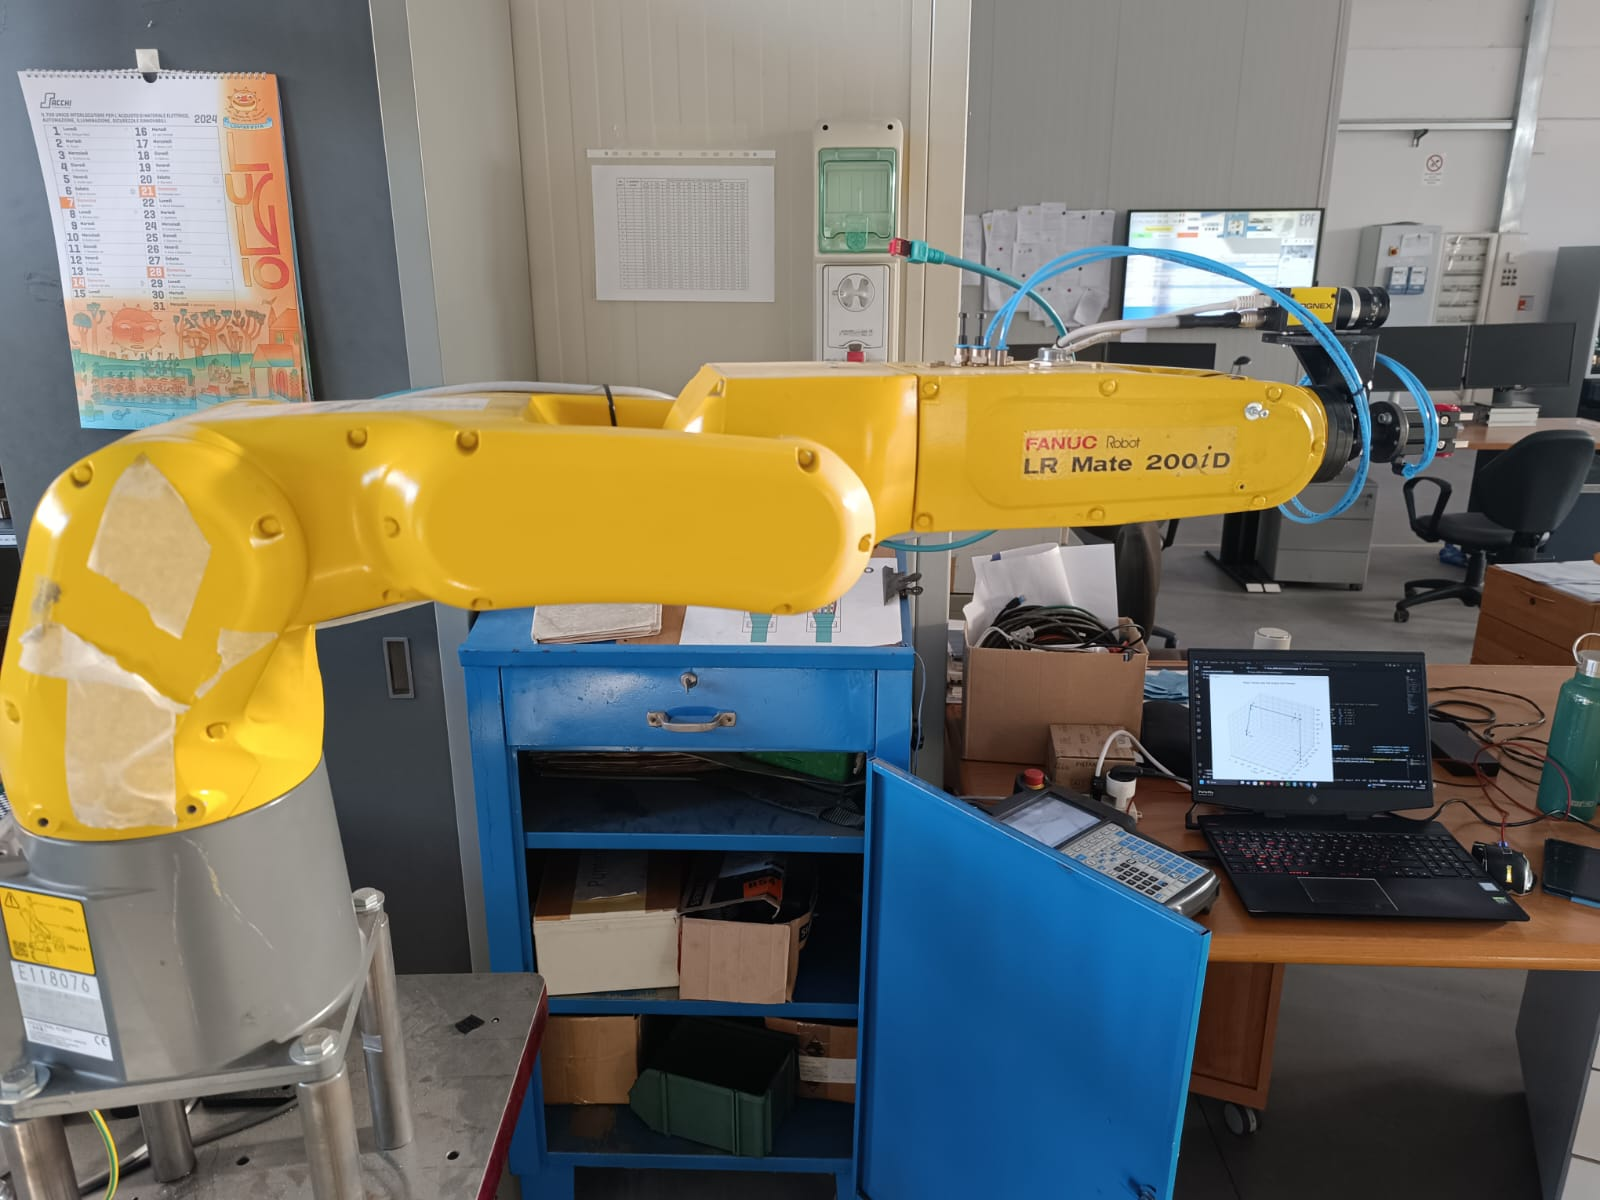
\includegraphics[width=\textwidth]{images/chapter4Images/full_fanuc_experimental_setup.png}
		\caption{Complete experimental setup showing workspace and ChArUco board.}
		\label{fig:setup_full}
	\end{subfigure}
	\hfill
	
	% ---------------- (c) ----------------
	\begin{subfigure}[t]{0.32\textwidth}
		\centering
		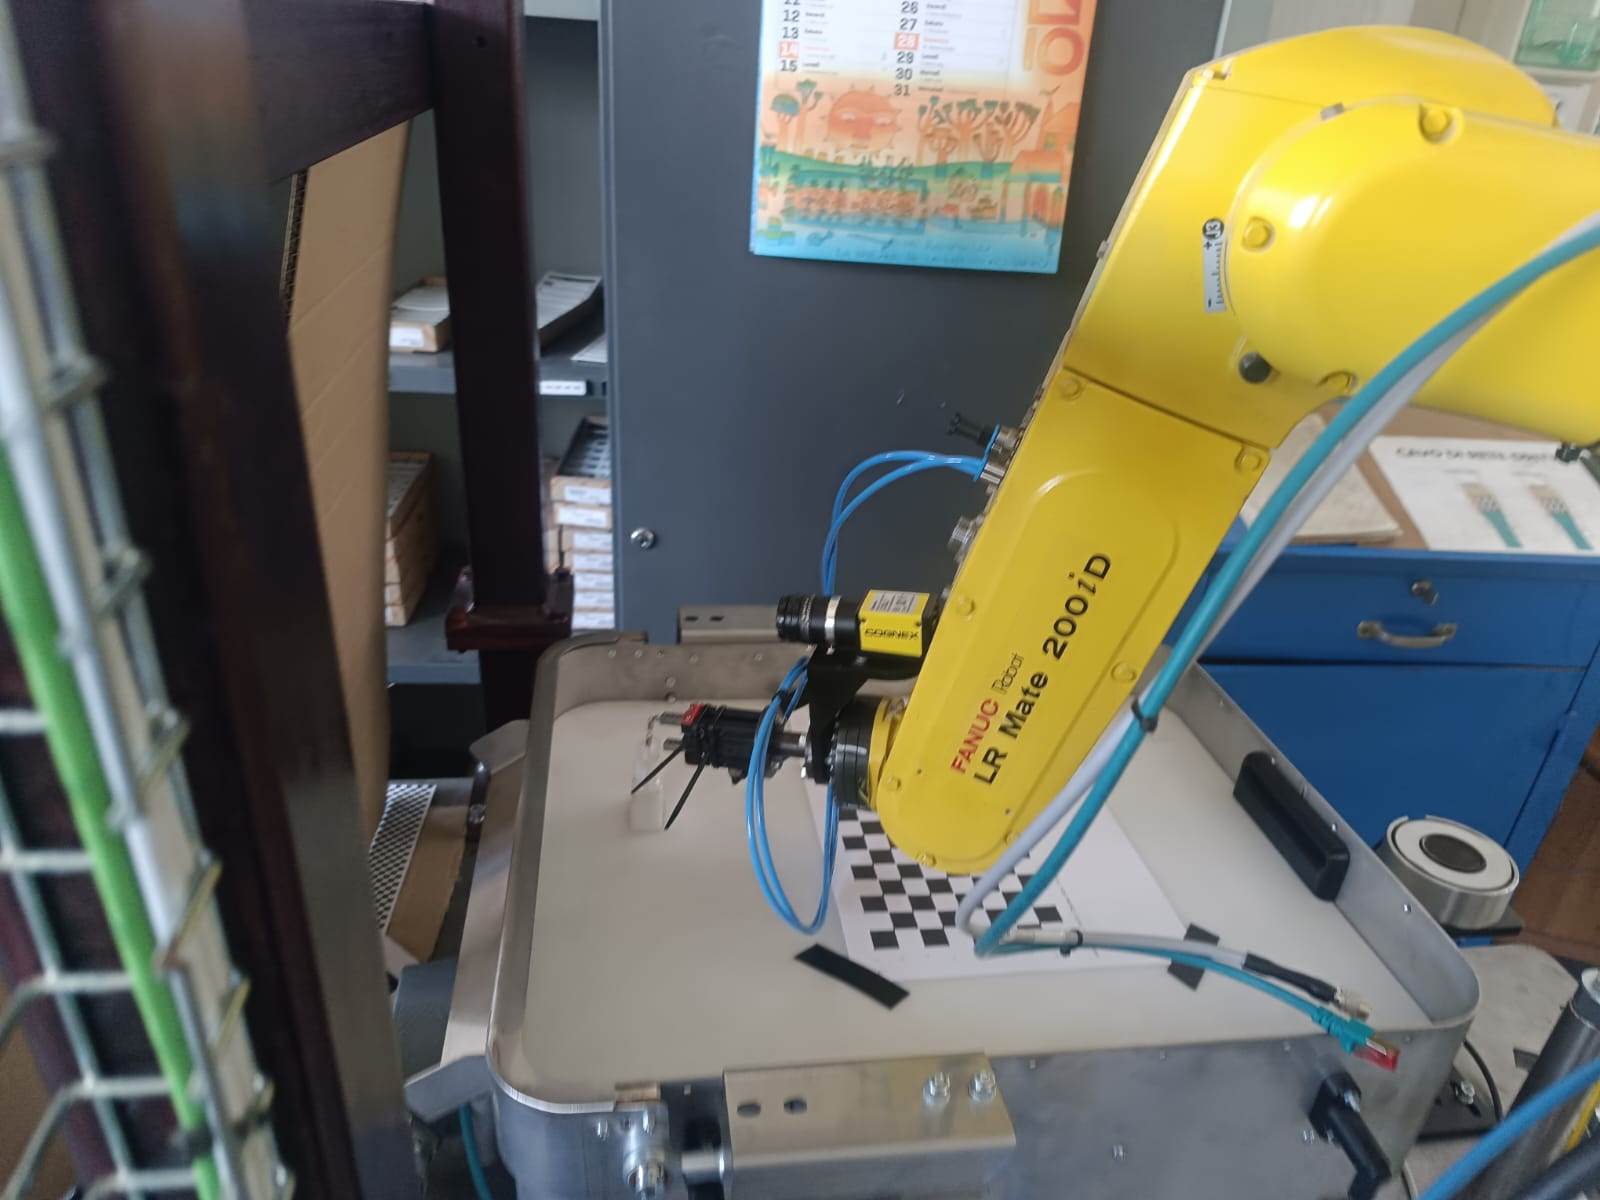
\includegraphics[width=\textwidth]{images/chapter4Images/experimental_setup_from_above.png}
		\caption{Top view highlighting geometric relations in the eye-in-hand setup.}
		\label{fig:setup_top}
	\end{subfigure}
	
	\caption{Experimental setup used for hand-eye calibration: (a) close-up view of the FANUC LR Mate 200iD with camera mounted on the end-effector, (b) full workspace configuration including calibration target placement, and (c) top-view perspective highlighting spatial relationships between robot, camera, and target.}
	\label{fig:experimental_setup}
\end{figure}

The robot is controlled by a FANUC R-30iB controller. Robot poses are defined
with respect to the base reference frame $\{B\}$ and are expressed as homogeneous
transformation matrices ${}^B_E\mathbf{T} \in SE(3)$ (Section~\ref{subsec:fk}).
In this work, poses were manually collected using the robot teach pendant.
Although this approach does not allow full automation of the acquisition process,
it provides direct control over the selection of robot configurations and ensures
the collection of sufficiently diverse and well-separated motions, as required by
the observability conditions discussed in Section~\ref{subsec:observability}.

The repeatability of the robot plays a crucial role in the calibration process,
as positioning inaccuracies directly propagate into the motion matrices
$\mathbf{A}_i$ used in the calibration equation~\eqref{eq:axxb}. The
$\pm$0.02\,mm repeatability of the LR Mate 200iD is well within the range
required for reliable hand-eye calibration in industrial applications.

% -- Figure [IMG-9]: Photo of the FANUC LR Mate 200iD in the experimental setup --
% (see figure suggestions at the end of this section)

% ---------------------------------------------------------------
\subsection{Camera System}
\label{subsec:camera_system}
% ---------------------------------------------------------------

The vision system is based on a \textbf{Cognex CAM-CIC-12-9C-IP67}
industrial area-scan camera. Its main specifications
are:

\begin{itemize}
    \item \textbf{Image sensor:} Sony IMX304, CMOS, global shutter
    \item \textbf{Resolution:} $4096 \times 3000$ pixels (12\,MP)
    \item \textbf{Sensor size:} 1.1\,inch diagonal
    \item \textbf{Pixel size:} $3.45 \times 3.45\,\mu$m
    \item \textbf{Bit depth:} 12\,bit
    \item \textbf{Maximum frame rate:} 9\,fps at full resolution
    \item \textbf{Data interface:} GigE Vision (M12 X-coded connector, PoE)
    \item \textbf{Protection rating:} IP67 (dust-proof and water-resistant,
    with IP67-rated lens tube)
    \item \textbf{Lens mount:} C-mount
\end{itemize}


\begin{figure}[htbp]
	\centering
	
	\begin{minipage}{0.48\textwidth}
		\centering
		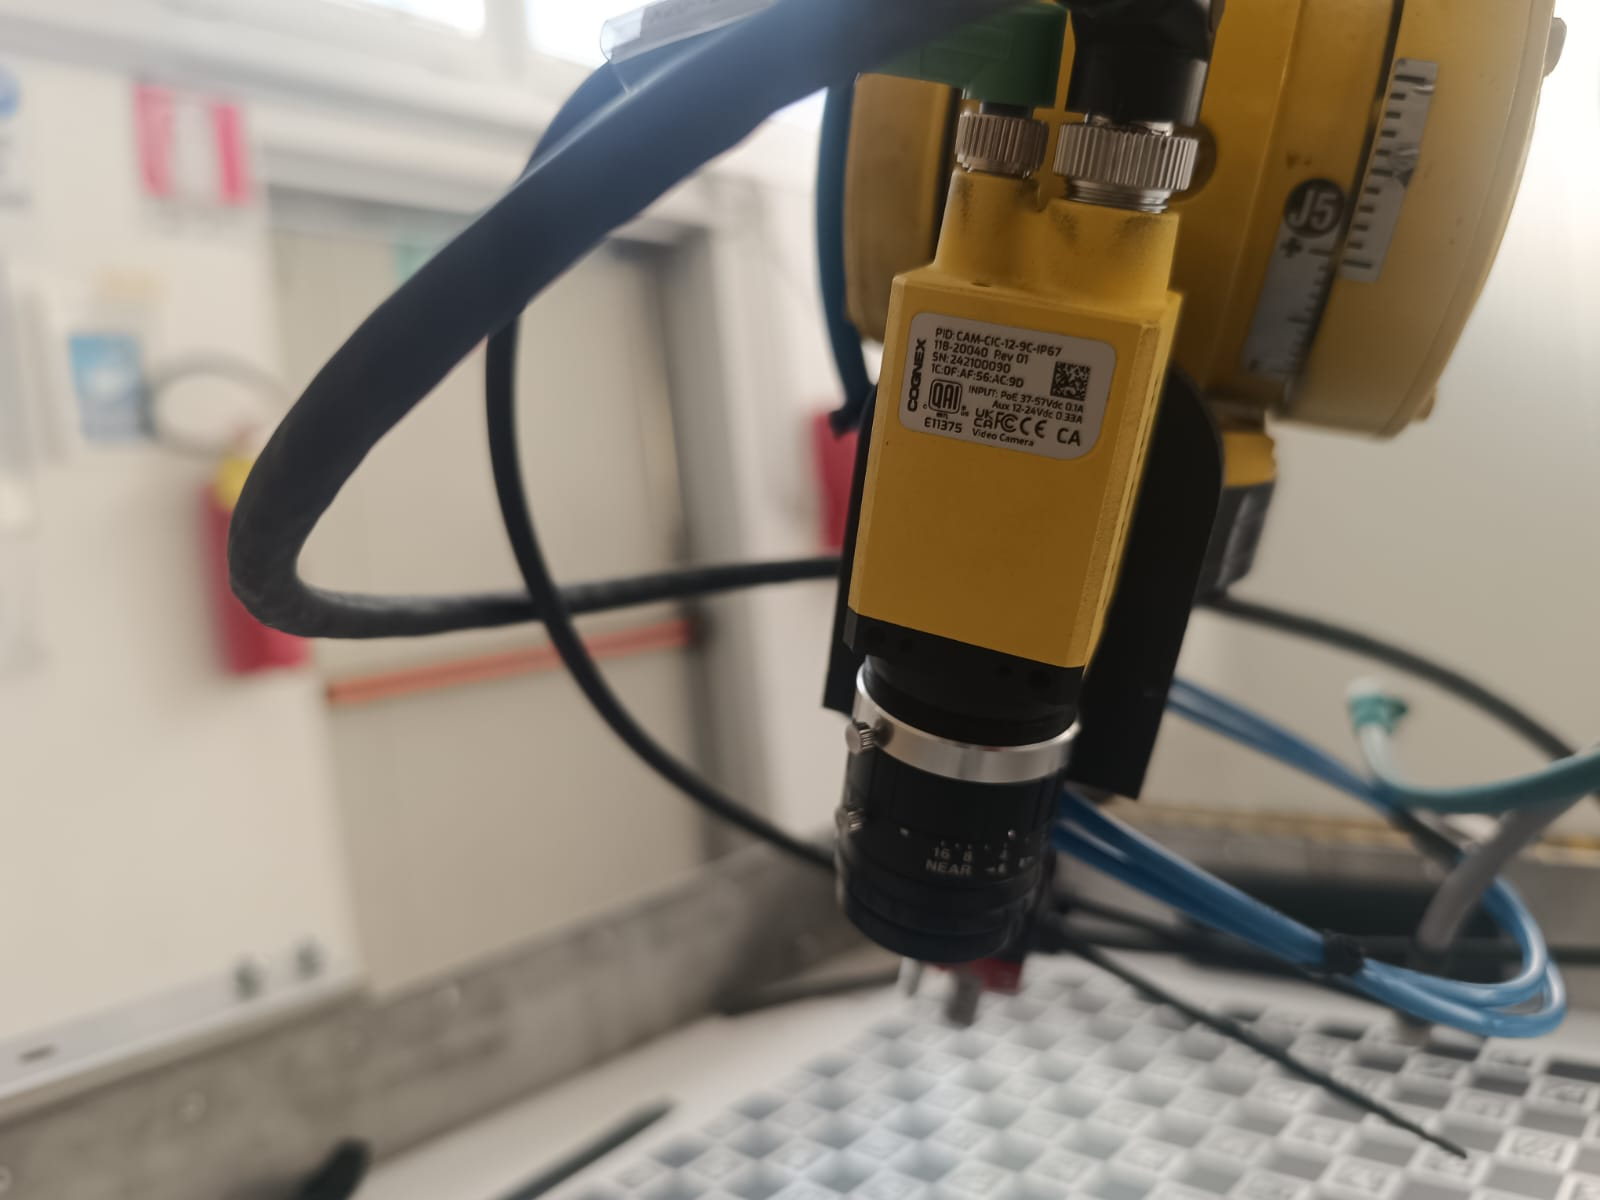
\includegraphics[width=\textwidth]{images/chapter4Images/Camera.png}
		\caption*{(a) Cognex camera}
	\end{minipage}
	\hfill
	\begin{minipage}{0.48\textwidth}
		\centering
		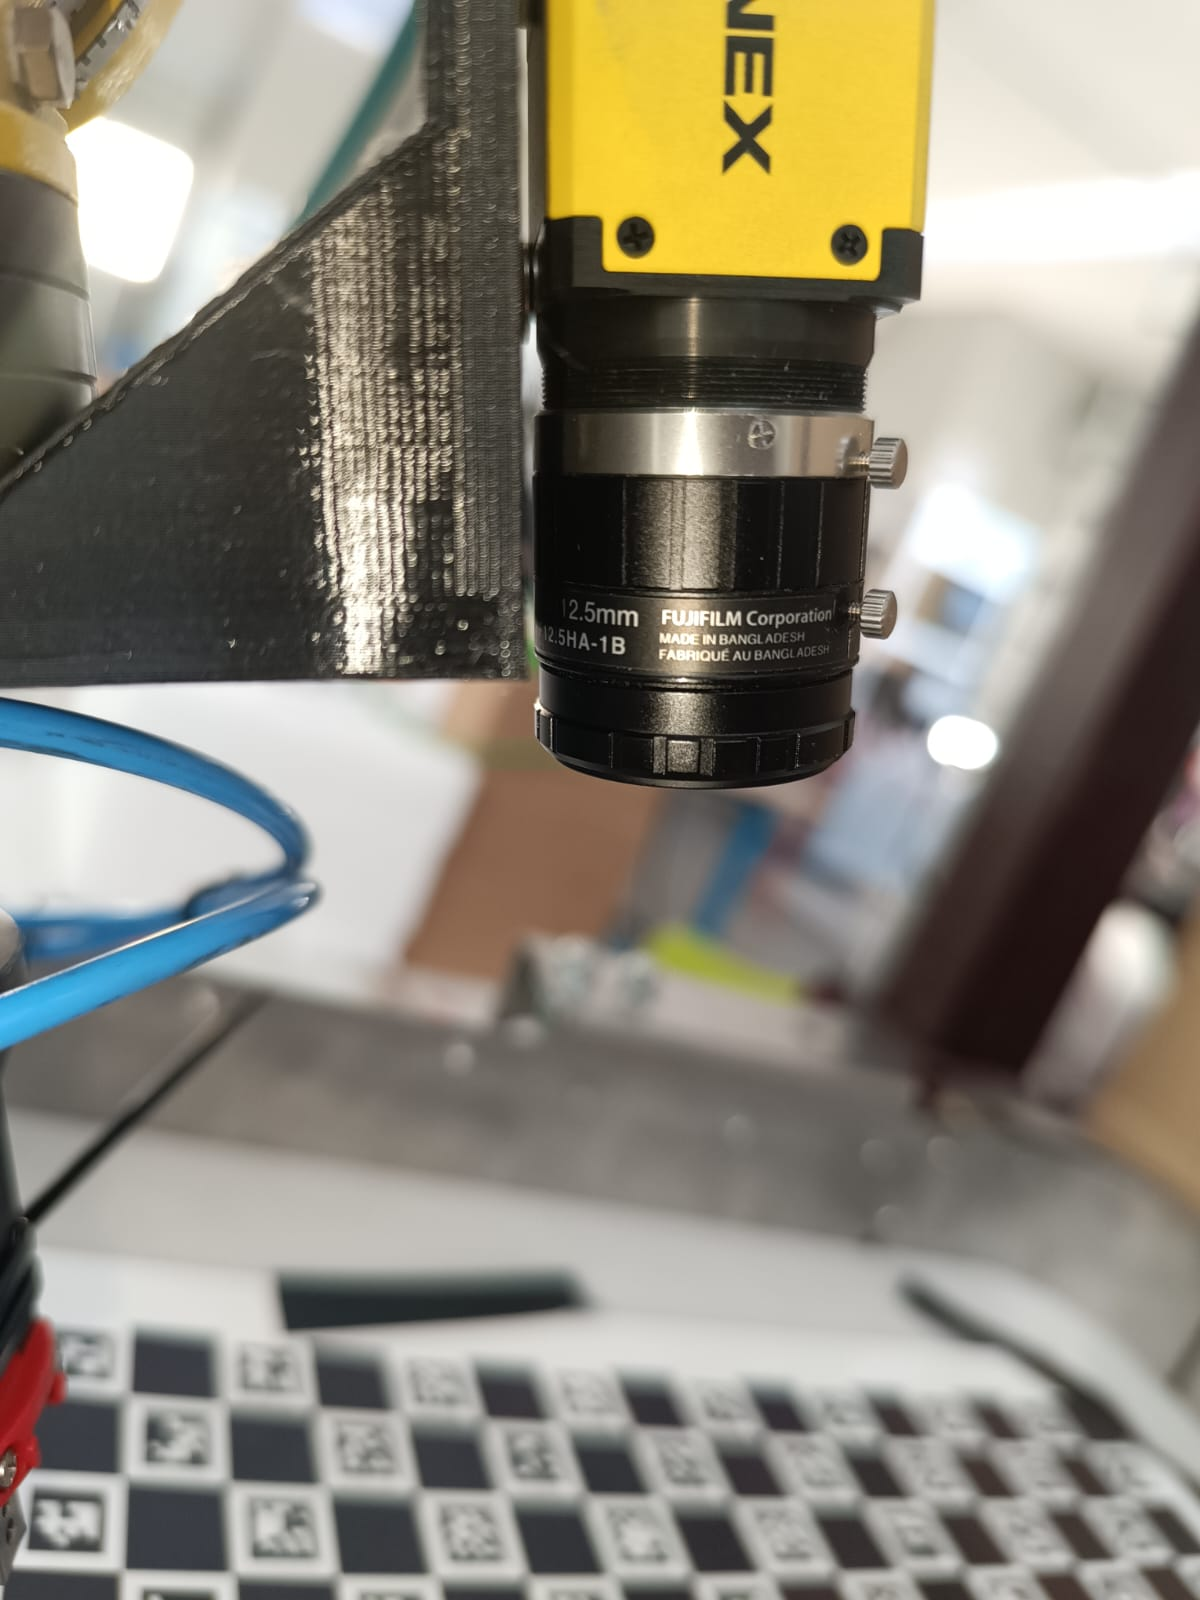
\includegraphics[width=\textwidth]{images/chapter4Images/Camera-end-effector-link.png}
		\caption*{(b) 3D-printed camera–end-effector mounting link}
	\end{minipage}
	
	\caption{Eye-in-hand vision setup: camera mounted on the robot end-effector using a custom 3D-printed adapter.}
	\label{fig:camera_setup}
\end{figure}


The camera is mounted directly on the robot end-effector, forming the
eye-in-hand configuration. The use of a \textit{global shutter} sensor is
particularly important in this context: unlike rolling shutter sensors, global
shutter sensors expose all pixels simultaneously, eliminating motion-induced
image distortions when the camera is in motion during image acquisition.

The high resolution of $4096 \times 3000$ pixels ensures that the corners of
the ChArUco calibration target (Section~\ref{subsec:calibration_target}) are
detected with sub-pixel accuracy, which is essential for precise pose estimation
and, consequently, for calibration accuracy.

Mounting the camera on the robot requires careful attention to mechanical
rigidity. Any relative motion between the camera and the end-effector flange
after calibration would directly invalidate the estimated transformation
$\mathbf{X}$. 

% ---------------------------------------------------------------
\subsection{Lens}
\label{subsec:lens}
% ---------------------------------------------------------------

The camera is equipped with a fixed focal length C-mount lens.
The lens was selected to provide a suitable working distance of approximately
30--40\,cm, ensuring that the entire calibration target is visible within the
camera's field of view while maintaining sufficient resolution for accurate
corner detection.

% ---------------------------------------------------------------
\subsection{Calibration Target}
\label{subsec:calibration_target}
% ---------------------------------------------------------------

A rigid \textbf{ChArUco board} \cite{garrido2014aruco} was used as the
calibration target. The board has physical dimensions of approximately
$262.5 \times 402.5$\,mm and is engraved on a metallic substrate, ensuring
dimensional stability and flatness under varying temperature and humidity
conditions.


The board consists of 15 x 23 squares checkerboard grid with embedded ArUco
fiducial markers \cite{garrido2014aruco}. Each checkerboard square has a side
length of 17.5\,mm, and each embedded ArUco marker has a side
length of 12\,mm.

\begin{figure}[htbp]
	\centering
	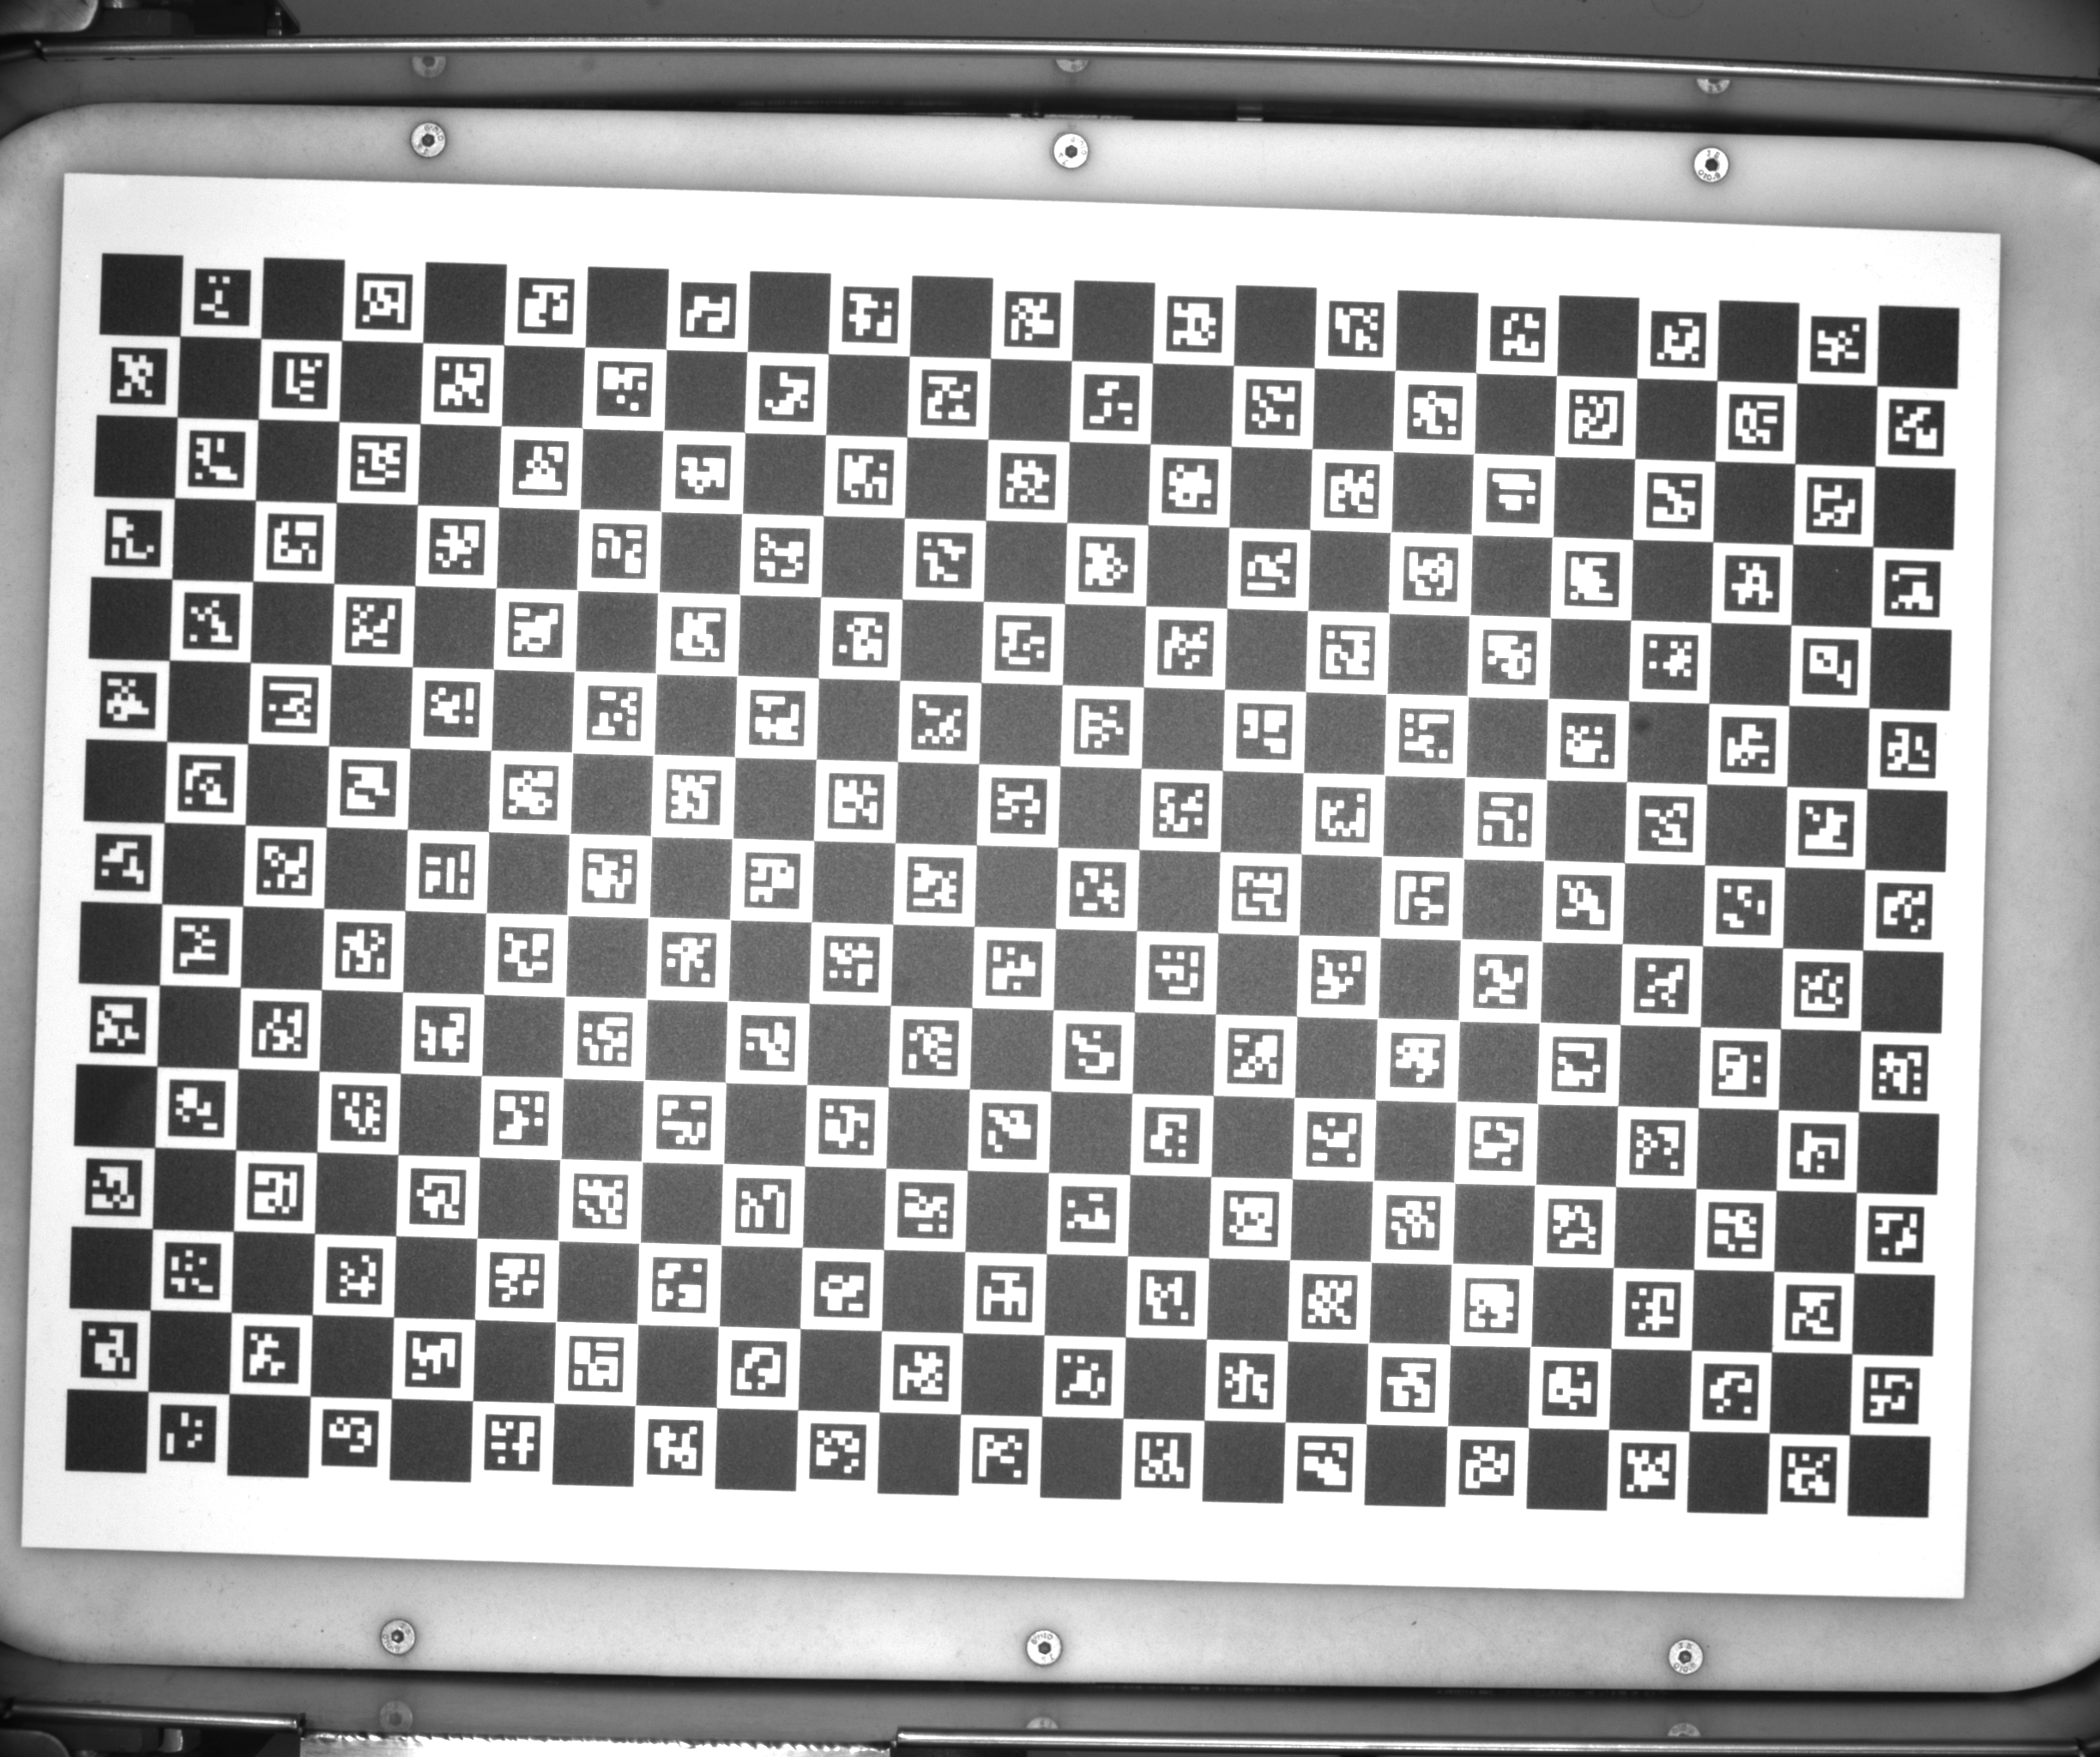
\includegraphics[width=0.45\textwidth]{images/chapter3Images/chessboardVertical.png}
	\caption{ChArUco calibration board used during the acquisition process. 
		The board combines a checkerboard pattern with embedded ArUco markers, 
		enabling robust and accurate corner detection for camera calibration and 
		pose estimation.}
	\label{fig:charuco_board}
\end{figure}
As shown in Figure~\ref{fig:charuco_board}, the ChArUco board combines the geometric precision of checkerboard corners with the robustness of fiducial marker detection.

ChArUco boards offer two complementary detection mechanisms:

\begin{itemize}
    \item \textbf{Checkerboard corners} provide high-accuracy sub-pixel
    localization, as corners can be refined to sub-pixel precision using
    standard corner refinement algorithms (e.g., OpenCV's
    \texttt{cornerSubPix}).

    \item \textbf{ArUco markers} provide reliable identification of each
    corner even under partial occlusions, strong perspective distortions,
    or non-uniform illumination, thanks to their binary encoding and
    error-correction capability \cite{garrido2014aruco}.
\end{itemize}

Compared to standard checkerboard targets, ChArUco boards therefore provide
robust detection even when portions of the pattern are not visible, reducing
the likelihood of incorrect corner assignments. The use of a rigid metallic
substrate — rather than a printed paper target — eliminates deformation-induced
errors that would otherwise introduce systematic bias in the estimated board
geometry.

During the acquisition process, multiple images of the calibration target are
captured from different robot poses. Observations with insufficient corner
detections or high reprojection errors are discarded.





\bigskip
\noindent\textit{Suggested figures for this section:}
\begin{itemize}
    \item \textbf{[IMG-9]} A photo of the FANUC LR Mate 200iD in your lab,
    with the camera mounted on the end-effector. Label the robot base frame
    $\{B\}$, end-effector frame $\{E\}$, and camera frame $\{C\}$ with
    arrows or overlaid text. This is the most important figure in the chapter.

    \item \textbf{[IMG-10]} A wider photo of the complete experimental setup,
    showing the robot, the ChArUco board on the table, and the cable routing
    to the GigE interface. Reviewers will look for this to understand the
    physical layout.

    
\end{itemize}


% ---------------------------------------------------------------
\section{Coordinate Frames Definition}
\label{sec:coordinate_frames}
% ---------------------------------------------------------------

In order to formulate the hand-eye calibration problem, it is necessary to
define the coordinate frames involved in the system and the transformations
between them. A clear and consistent notation is essential to correctly
interpret both robot and camera data, and to establish the geometric
relationships required for calibration \cite{craig2005introduction,
siciliano2009robotics}.

In this work, four coordinate frames are considered, as illustrated in
Figure~\ref{fig:coordinate_frames}:

\begin{itemize}
    \item $\{B\}$ — the \textbf{robot base frame}, fixed to the robot base;
    \item $\{E\}$ — the \textbf{end-effector frame}, attached to the robot flange;
    \item $\{C\}$ — the \textbf{camera frame}, centred at the optical centre of
    the camera;
    \item $\{T\}$ — the \textbf{target frame}, attached to the ChArUco board.
\end{itemize}

All transformations between frames are expressed as homogeneous transformation
matrices $\mathbf{T} \in SE(3)$ (Section~\ref{subsec:homogeneous}), where the
left superscript denotes the destination frame and the left subscript denotes
the source frame. For example, ${}^A_B\mathbf{T}$ maps a point expressed in
frame $\{B\}$ into frame $\{A\}$.

% ---------------------------------------------------------------
\subsection{Robot Base Frame \texorpdfstring{$\{B\}$}{B}}
\label{subsec:frame_base}
% ---------------------------------------------------------------

The robot base frame $\{B\}$ is a fixed reference frame rigidly attached to the
base of the FANUC LR Mate 200iD manipulator. It serves as the global reference
for all robot motions. The robot controller computes and provides, at each
configuration $\mathbf{q}$, the pose of the end-effector with respect to this
frame via forward kinematics (Section~\ref{subsec:fk}):

\begin{equation}
    {}^B_E\mathbf{T}(\mathbf{q}) =
    \begin{bmatrix} {}^B_E\mathbf{R} & {}^B\mathbf{t}_E \\
    \mathbf{0}^{\top} & 1 \end{bmatrix} \in SE(3)
    \label{eq:T_BE}
\end{equation}

\noindent This matrix encodes the full pose — position and orientation — of the
end-effector frame $\{E\}$ relative to $\{B\}$.The robot controller provides Cartesian pose measurements, which are converted into homogeneous transformation matrices for subsequent processing.


% ---------------------------------------------------------------
\subsection{End-Effector Frame \texorpdfstring{$\{E\}$}{E}}
\label{subsec:frame_ee}
% ---------------------------------------------------------------

The end-effector frame $\{E\}$ is attached to the robot tool flange. It moves
rigidly with the robot and constitutes the reference frame of the tool to which
the camera is mounted.

In the eye-in-hand configuration adopted in this work, the camera is rigidly
fixed to the end-effector. Therefore, the transformation between $\{E\}$ and
the camera frame $\{C\}$:

\begin{equation}
    \mathbf{X} = {}^E_C\mathbf{T} =
    \begin{bmatrix} {}^E_C\mathbf{R} & {}^E\mathbf{t}_C \\
    \mathbf{0}^{\top} & 1 \end{bmatrix} \in SE(3)
    \label{eq:X_EC}
\end{equation}

\noindent is \textit{constant} for all robot configurations, provided that the
camera mounting does not change. Estimating $\mathbf{X}$ is precisely the
objective of the hand-eye calibration procedure. % TODO: update chapter reference

% ---------------------------------------------------------------
\subsection{Camera Frame \texorpdfstring{$\{C\}$}{C}}
\label{subsec:frame_camera}
% ---------------------------------------------------------------

The camera frame $\{C\}$ has its origin at the optical centre of the Cognex
CAM-CIC-12-9C-IP67 camera. Following the standard computer vision convention
\cite{hartley2004multiple}:

\begin{itemize}
    \item the $Z_C$-axis points along the optical axis (i.e.\ forward,
    towards the scene);
    \item the $X_C$-axis points to the right along the image sensor plane;
    \item the $Y_C$-axis points downward along the image sensor plane.
\end{itemize}

\noindent The pose of the calibration target $\{T\}$ expressed in $\{C\}$
(see Section~\ref{subsec:frame_target}) is the direct output of the
PnP-based pose estimation described in Section~\ref{subsec:pnp_opencv}.

% ---------------------------------------------------------------
\subsection{Target Frame \texorpdfstring{$\{T\}$}{T}}
\label{subsec:frame_target}
% ---------------------------------------------------------------

The target frame $\{T\}$ is attached to the ChArUco board used during the
calibration procedure (Section~\ref{subsec:calibration_target}). Its origin is
placed at a reference corner of the board, with axes aligned with the board
geometry as established during the board definition in OpenCV .

At each robot pose $i$, the pose of $\{T\}$ with respect to the camera frame
is estimated from the detected ChArUco corners via \texttt{cv::solvePnP()}:

\begin{equation}
    {}^C_T\mathbf{T}^{(i)} =
    \begin{bmatrix} {}^C_T\mathbf{R}^{(i)} & {}^C\mathbf{t}_T^{(i)} \\
    \mathbf{0}^{\top} & 1 \end{bmatrix} \in SE(3)
    \label{eq:T_CT}
\end{equation}

\noindent In the eye-in-hand configuration, the board is \textit{fixed} in the
environment, so ${}^C_T\mathbf{T}^{(i)}$ changes at every robot pose as the
camera moves with the end-effector.

% ---------------------------------------------------------------
\subsection{Transformation Relationships and Calibration Equation}
\label{subsec:frame_relationships}
% ---------------------------------------------------------------

The four frames define a closed kinematic chain that must be consistent for any
pair of robot poses $i$ and $j$:

\begin{equation}
    {}^B_E\mathbf{T}^{(i)} \cdot {}^E_C\mathbf{T} \cdot {}^C_T\mathbf{T}^{(i)}
    =
    {}^B_E\mathbf{T}^{(j)} \cdot {}^E_C\mathbf{T} \cdot {}^C_T\mathbf{T}^{(j)}
    \label{eq:chain_consistency}
\end{equation}

\noindent Rearranging equation~\eqref{eq:chain_consistency} yields the
hand-eye calibration equation introduced in Section~\ref{subsec:hec_formulation}:

\begin{equation}
    \mathbf{A}_{ij} \mathbf{X} = \mathbf{X} \mathbf{B}_{ij}
    \label{eq:axb_frames}
\end{equation}

\noindent where the motion matrices $\mathbf{A}_{ij}$ and $\mathbf{B}_{ij}$
are computed from consecutive pose observations as:

\begin{align}
    \mathbf{A}_{ij} &=
    \left({}^B_E\mathbf{T}^{(i)}\right)^{-1}
    {}^B_E\mathbf{T}^{(j)}
    \label{eq:A_ij} \\[4pt]
    \mathbf{B}_{ij} &=
    {}^C_T\mathbf{T}^{(i)}
    \left({}^C_T\mathbf{T}^{(j)}\right)^{-1}
    \label{eq:B_ij}
\end{align}

\noindent using the inverse formula from equation~\eqref{eq:T_inverse}.
The quantity $\mathbf{A}_{ij}$ represents the relative motion of the
end-effector in the base frame, obtained from the robot controller.
The quantity $\mathbf{B}_{ij}$ represents the corresponding relative motion
of the camera as seen by the fixed calibration target, obtained from
pose estimation.

By collecting $n$ such motion pairs $\{(\mathbf{A}_{ij},
\mathbf{B}_{ij})\}$, the calibration pipeline solves for the unknown
$\mathbf{X} = {}^E_C\mathbf{T}$ using the methods described in
Section~\ref{subsec:hec_methods}.

A summary of the four frames and their associated transformations is provided
in Table~\ref{tab:frames_summary}.

\begin{table}[h]
    \centering
    \caption{Coordinate frames and associated transformations.}
    \label{tab:frames_summary}
    \begin{tabular}{llll}
        \toprule
        \textbf{Frame} & \textbf{Notation} & \textbf{Transformation} &
        \textbf{Source} \\
        \midrule
        Robot base      & $\{B\}$ & — (world reference)           & Fixed \\
        End-effector    & $\{E\}$ & ${}^B_E\mathbf{T}(\mathbf{q})$
                                  & Forward kinematics \\
        Camera          & $\{C\}$ & $\mathbf{X} = {}^E_C\mathbf{T}$
                                  & \textbf{To be calibrated} \\
        Target (board)  & $\{T\}$ & ${}^C_T\mathbf{T}^{(i)}$
                                  & Pose estimation (PnP) \\
        \bottomrule
    \end{tabular}
\end{table}


\begin{figure}[htbp]
    \centering
    \begin{tikzpicture}[
        every node/.style = {font=\small},
        frame/.style     = {draw, rounded corners=4pt, minimum width=2.2cm,
                            minimum height=0.9cm, align=center},
        transf/.style    = {-Stealth, thick},
        unknown/.style   = {-Stealth, thick, dashed, red!70!black},
        label/.style     = {font=\footnotesize, fill=white, inner sep=2pt},
    ]

    % ---- nodes (frames) ----
    \node[frame, fill=gray!15]               (B) {$\{B\}$\\Base};
    \node[frame, fill=blue!12,
          right=3.2cm of B]                  (E) {$\{E\}$\\End-effector};
    \node[frame, fill=orange!20,
          right=3.2cm of E]                  (C) {$\{C\}$\\Camera};
    \node[frame, fill=green!15,
          below=2.2cm of C]                  (T) {$\{T\}$\\Target};

    % ---- robot arm sketch (simplified) between B and E ----
    \draw[thick, gray!60, line cap=round]
        ($(B.east)+(0,0.15)$) -- ++(0.5,0.3) -- ++(0.8,0) -- ++(0.5,-0.3);
    \draw[thick, gray!60, line cap=round]
        ($(B.east)+(0,-0.15)$) -- ++(0.5,-0.2) -- ++(0.8,0) -- ++(0.5,0.2);

    % ---- known transformations ----
    \draw[transf] (B.east)  -- node[label, above]{${}^B_E\mathbf{T}(\mathbf{q})$}
                                node[label, below]{\textit{fwd.\ kinematics}} (E.west);

    \draw[transf] (C.south) -- node[label, right]{${}^C_T\mathbf{T}^{(i)}$}
                                node[label, left]{\textit{pose estimation}} (T.north);

    % ---- unknown transformation (dashed red) ----
    \draw[unknown] (E.east) -- node[label, above]{$\mathbf{X} = {}^E_C\mathbf{T}$}
                                node[label, below]{\textit{to calibrate}} (C.west);

    

    % ---- legend ----
    \node[anchor=north west, font=\footnotesize] at ($(B.south west)-(0,0.7)$) {
        \begin{tabular}{@{}ll@{}}
            \tikz\draw[transf] (0,0)--(0.5,0); & Known transformation \\[2pt]
            \tikz\draw[unknown](0,0)--(0.5,0); & Unknown (hand-eye transformationt) \\
        \end{tabular}
    };

    \end{tikzpicture}
    \caption{The four coordinate frames involved in the eye-in-hand calibration
             setup and the rigid transformations between them. The unknown
             transformation $\mathbf{X} = {}^E_C\mathbf{T}$ (dashed red) is
             estimated by the calibration procedure from the known robot motions
             $\mathbf{A}_{ij}$ and the camera-observed target motions
             $\mathbf{B}_{ij}$.}
    \label{fig:coordinate_frames}
\end{figure}





\section{Data Acquisition Pipeline}
\label{sec:acquisition_pipeline}

This section describes the data acquisition process used to collect the
information required for hand-eye calibration. The pipeline combines robot
motion, image acquisition, ChArUco feature detection, pose estimation, and
data validation in order to produce the motion pairs
$\{(\mathbf{A}_{ij}, \mathbf{B}_{ij})\}$ used as input to the calibration
algorithm (Section~\ref{subsec:hec_formulation}). An overview of the pipeline
is illustrated in Figure~\ref{fig:acquisition_pipeline}.

% ---------------------------------------------------------------
\subsection{Robot Pose Acquisition}
\label{subsec:robot_pose_acq}
% ---------------------------------------------------------------

The FANUC LR Mate 200iD is moved to a sequence of $n$ distinct configurations
in order to acquire a diverse set of observations. At each configuration
$\mathbf{q}^{(k)}$, the pose of the end-effector with respect to the robot
base frame is recorded:

\begin{equation}
	{}^B_E\mathbf{T}^{(k)} = {}^B_E\mathbf{T}\!\left(\mathbf{q}^{(k)}\right)
	\in SE(3), \qquad k = 1, \dots, n
	\label{eq:recorded_poses}
\end{equation}

\noindent The robot controller provides the Cartesian pose of the end-effector, which is subsequently converted into a homogeneous transformation matrix at the moment the robot reaches a stable,
stationary configuration.

In this work, robot poses were manually collected using the teach pendant of
the FANUC LR Mate 200iD. Although this approach does not allow full automation
of the data acquisition, it gives direct control over the selection of robot
configurations. Poses are chosen to ensure sufficient variation in both
position and orientation. In particular:

\begin{itemize}
	\item rotations are distributed across multiple non-parallel axes;
	\item the magnitude of each rotation is large enough to be distinguishable
	from measurement noise;
	\item pure translational motions without rotational components are avoided;
	\item the calibration target remains visible in the camera field of view
	at each pose.
\end{itemize}

\noindent In practice, datasets containing approximately 15–20 sufficiently diverse poses are often adequate to obtain stable calibration estimates, although the exact number depends on the motion diversity and measurement quality.

% ---------------------------------------------------------------
\subsection{Image Acquisition}
\label{subsec:image_acq}
% ---------------------------------------------------------------

For each robot pose $k$, a single image of the ChArUco calibration target is
captured by the Cognex CAM-CIC-12-9C-IP67 camera mounted on the end-effector.
Since the system operates in an eye-in-hand configuration
(Section~\ref{subsec:eye_in_hand}), the camera moves with the robot while the
calibration target remains fixed.

Image acquisition is performed after the robot has reached a complete stop at
each target pose, ensuring that motion-induced blur is minimised and that the
recorded end-effector pose ${}^B_E\mathbf{T}^{(k)}$ and the corresponding
image are temporally consistent. Any mismatch between these two quantities
directly corrupts the motion pair $(\mathbf{A}_{ij}, \mathbf{B}_{ij})$ and
must therefore be avoided. The global shutter of the Sony IMX304 sensor
(Section~\ref{subsec:camera_system}) additionally eliminates rolling-shutter
artefacts that would otherwise distort the apparent geometry of the target
even at rest.

% ---------------------------------------------------------------
\subsection{ChArUco Feature Detection}
\label{subsec:feature_detection}
% ---------------------------------------------------------------

Once an image is acquired, ChArUco corners are extracted using the OpenCV
\texttt{aruco} module \cite{garrido2014aruco, bradski2008learning}. The
detection follows the three-stage procedure — ArUco marker detection,
ChArUco corner interpolation, and sub-pixel refinement via
\texttt{cv::cornerSubPix()} — described in detail in
Section~\ref{subsec:intr_detection} in the context of intrinsic calibration.
The same procedure is applied here; when the intrinsic matrix $\mathbf{K}$
and distortion coefficients are available, the corner interpolation benefits
from an approximate pose refinement step rather than falling back to the
homography-based mode.

The output of the detection stage is a set of $m_k$ ChArUco corner
coordinates in the image, $\{\tilde{\mathbf{p}}_j^{(k)}\}_{j=1}^{m_k}$,
and their corresponding 3D positions on the board,
$\{\mathbf{P}_j\}_{j=1}^{m_k}$, expressed in the target frame $\{T\}$.

% ---------------------------------------------------------------
\subsection{Pose Estimation and Data Validation}
\label{subsec:pose_est_filtering}
% ---------------------------------------------------------------

The 2D--3D correspondences obtained from the detection stage are used to
estimate the pose of the calibration target with respect to the camera frame,
${}^C_T\mathbf{T}^{(k)} \in SE(3)$, via the P$n$P algorithm. The full
formulation — including the reprojection minimisation objective, the use of
\texttt{cv::solvePnP()} with Levenberg--Marquardt refinement, and the
Rodrigues conversion to a homogeneous transformation — is given in
Section~\ref{subsec:extr_pose_est}, where it is presented in the context of
extrinsic calibration.

Not all acquired images yield reliable pose estimates. An observation $k$ is
rejected from the dataset if any of the following conditions is met:

\begin{itemize}
	\item \textbf{Insufficient corners:} fewer than $m_{\min}$ ChArUco corners
	are detected, making the P$n$P problem underdetermined or degenerate.
	
	\item \textbf{High reprojection error:} the mean reprojection error of the
	pose estimate exceeds a threshold $\epsilon_{\max} \in [0.8, 1.5]$\,px, depending on sensor resolution and
	working distance.
	
	\item \textbf{Poor image quality:} motion blur, overexposure, or partial
	occlusion of the target, detected by manual inspection and automated
	image-quality metrics.
\end{itemize}

\noindent After filtering, the validated dataset consists of $n' \leq n$
accepted observation pairs $\bigl({}^B_E\mathbf{T}^{(k)},\,
{}^C_T\mathbf{T}^{(k)}\bigr)$.

% ---------------------------------------------------------------
\subsection{Data Pairing and Input to Calibration}
\label{subsec:data_pairing}
% ---------------------------------------------------------------

From the $n'$ validated observations, relative motion pairs
$(\mathbf{A}_{ij}, \mathbf{B}_{ij})$ are computed for each pair of distinct
poses $(i,j)$, as defined in equations~\eqref{eq:A_ij}--\eqref{eq:B_ij}.
In practice, consecutive pairs $(i,\,i{+}1)$ are preferred over all
$\binom{n'}{2}$ combinations to limit the dataset size while maintaining
diversity and avoiding degenerate near-identity motion matrices. The complete
dataset $\{(\mathbf{A}_{ij}, \mathbf{B}_{ij})\}$ constitutes the input to the
hand-eye calibration algorithms described in Section~\ref{subsec:hec_methods},
which solve for the unknown transformation $\mathbf{X} = {}^E_C\mathbf{T}$.

The overall pipeline was initially prototyped in \textbf{Python} using OpenCV
\cite{bradski2008learning} and later reimplemented in \textbf{C\#} for
integration within the \textit{Cognex Designer} industrial vision environment,
enabling evaluation under realistic industrial conditions.

\begin{figure}[htbp]
    \centering
    \begin{tikzpicture}[
        node distance  = 0.6cm and 1.8cm,
        box/.style     = {draw, rounded corners=5pt, minimum width=3.8cm,
                          minimum height=0.85cm, align=center, font=\small,
                          fill=blue!6},
        decision/.style= {draw, diamond, aspect=2.2, font=\small,
                          fill=orange!12, align=center,
                          minimum width=3.8cm, minimum height=0.85cm},
        reject/.style  = {draw, rounded corners=5pt, minimum width=2.4cm,
                          minimum height=0.7cm, align=center, font=\small,
                          fill=red!10},
        arr/.style     = {-Stealth, thick},
        label/.style   = {font=\footnotesize, fill=white, inner sep=1pt},
    ]

    \node[box]      (pose)   {Robot pose acquisition\\
                               \footnotesize${}^B_E\mathbf{T}^{(k)}$ from controller};
    \node[box,  below=of pose]   (img)    {Image acquisition\\
                               \footnotesize Cognex CAM-CIC-12-9C-IP67};
    \node[box,  below=of img]    (detect) {ChArUco feature detection\\
                               \footnotesize \texttt{detectBoard()} + \texttt{cornerSubPix()}};
    \node[decision, below=of detect] (valid1)
    {Enough\\corners?};
    \node[reject, right=1.6cm of valid1] (rej1) {Reject image};
    \node[box,  below=of valid1] (pnp)    {Pose estimation (PnP)\\
                               \footnotesize \texttt{solvePnP()} $\rightarrow$
                               ${}^C_T\mathbf{T}^{(k)}$};
    \node[decision, below=of pnp] (valid2) {Reprojection\\error $\leq \epsilon_{\max}$?};
    \node[reject, right=1.6cm of valid2] (rej2) {Reject image};
    \node[box,  below=of valid2] (store)  {Store validated pair\\
                               \footnotesize $({}^B_E\mathbf{T}^{(k)},\;
                               {}^C_T\mathbf{T}^{(k)})$};
    \node[decision, below=of store] (more)  {More poses\\needed?};
    \node[box,  below=of more]   (pair)   {Compute motion pairs\\
                               \footnotesize $(\mathbf{A}_{ij},\,\mathbf{B}_{ij})$
                               via Eq.~\eqref{eq:A_ij}--\eqref{eq:B_ij}};
    \node[box,  below=of pair]   (calib)  {Hand-eye calibration\\
                               \footnotesize Solve $\mathbf{A}_{ij}\mathbf{X}
                               = \mathbf{X}\mathbf{B}_{ij}$};

    % Arrows (main flow)
    \draw[arr] (pose)   -- (img);
    \draw[arr] (img)    -- (detect);
    \draw[arr] (detect) -- (valid1);
    \draw[arr] (valid1) -- node[label,left]{yes} (pnp);
    \draw[arr] (valid1) -- node[label,above]{no}  (rej1);
    \draw[arr] (pnp)    -- (valid2);
    \draw[arr] (valid2) -- node[label,left]{yes} (store);
    \draw[arr] (valid2) -- node[label,above]{no}  (rej2);
    \draw[arr] (store)  -- (more);
    \draw[arr] (more)   -- node[label,left]{no}  (pair);
    \draw[arr] (pair)   -- (calib);
    % Loop-back arrow for "more poses needed"
    \draw[arr] (more.east) -- ++(1.1,0)
        |- node[label,right]{yes} (pose.east);
    \end{tikzpicture}
    \caption{Data acquisition pipeline for hand-eye calibration. At each robot
             pose, an image is captured and processed through ChArUco detection
             and PnP pose estimation. Observations failing the quality criteria
             are discarded. The validated dataset is used to compute the motion
             pairs $(\mathbf{A}_{ij}, \mathbf{B}_{ij})$ for the calibration
             algorithm.}
    \label{fig:acquisition_pipeline}
\end{figure}

